\hypertarget{md5_8cpp}{
\section{md5/md5.cpp File Reference}
\label{md5_8cpp}\index{md5/md5.cpp@{md5/md5.cpp}}
}
Diese Funktionen liefern die Moeglichkeit, einen MD5-Hash eines beliebigen String zu generieren. 

{\tt \#include $<$stdlib.h$>$}\par
{\tt \#include $<$string.h$>$}\par
{\tt \#include $<$sys/types.h$>$}\par
{\tt \#include \char`\"{}md5.h\char`\"{}}\par
{\tt \#include \char`\"{}md5\_\-loc.h\char`\"{}}\par


Include dependency graph for md5.cpp:\nopagebreak
\begin{figure}[H]
\begin{center}
\leavevmode
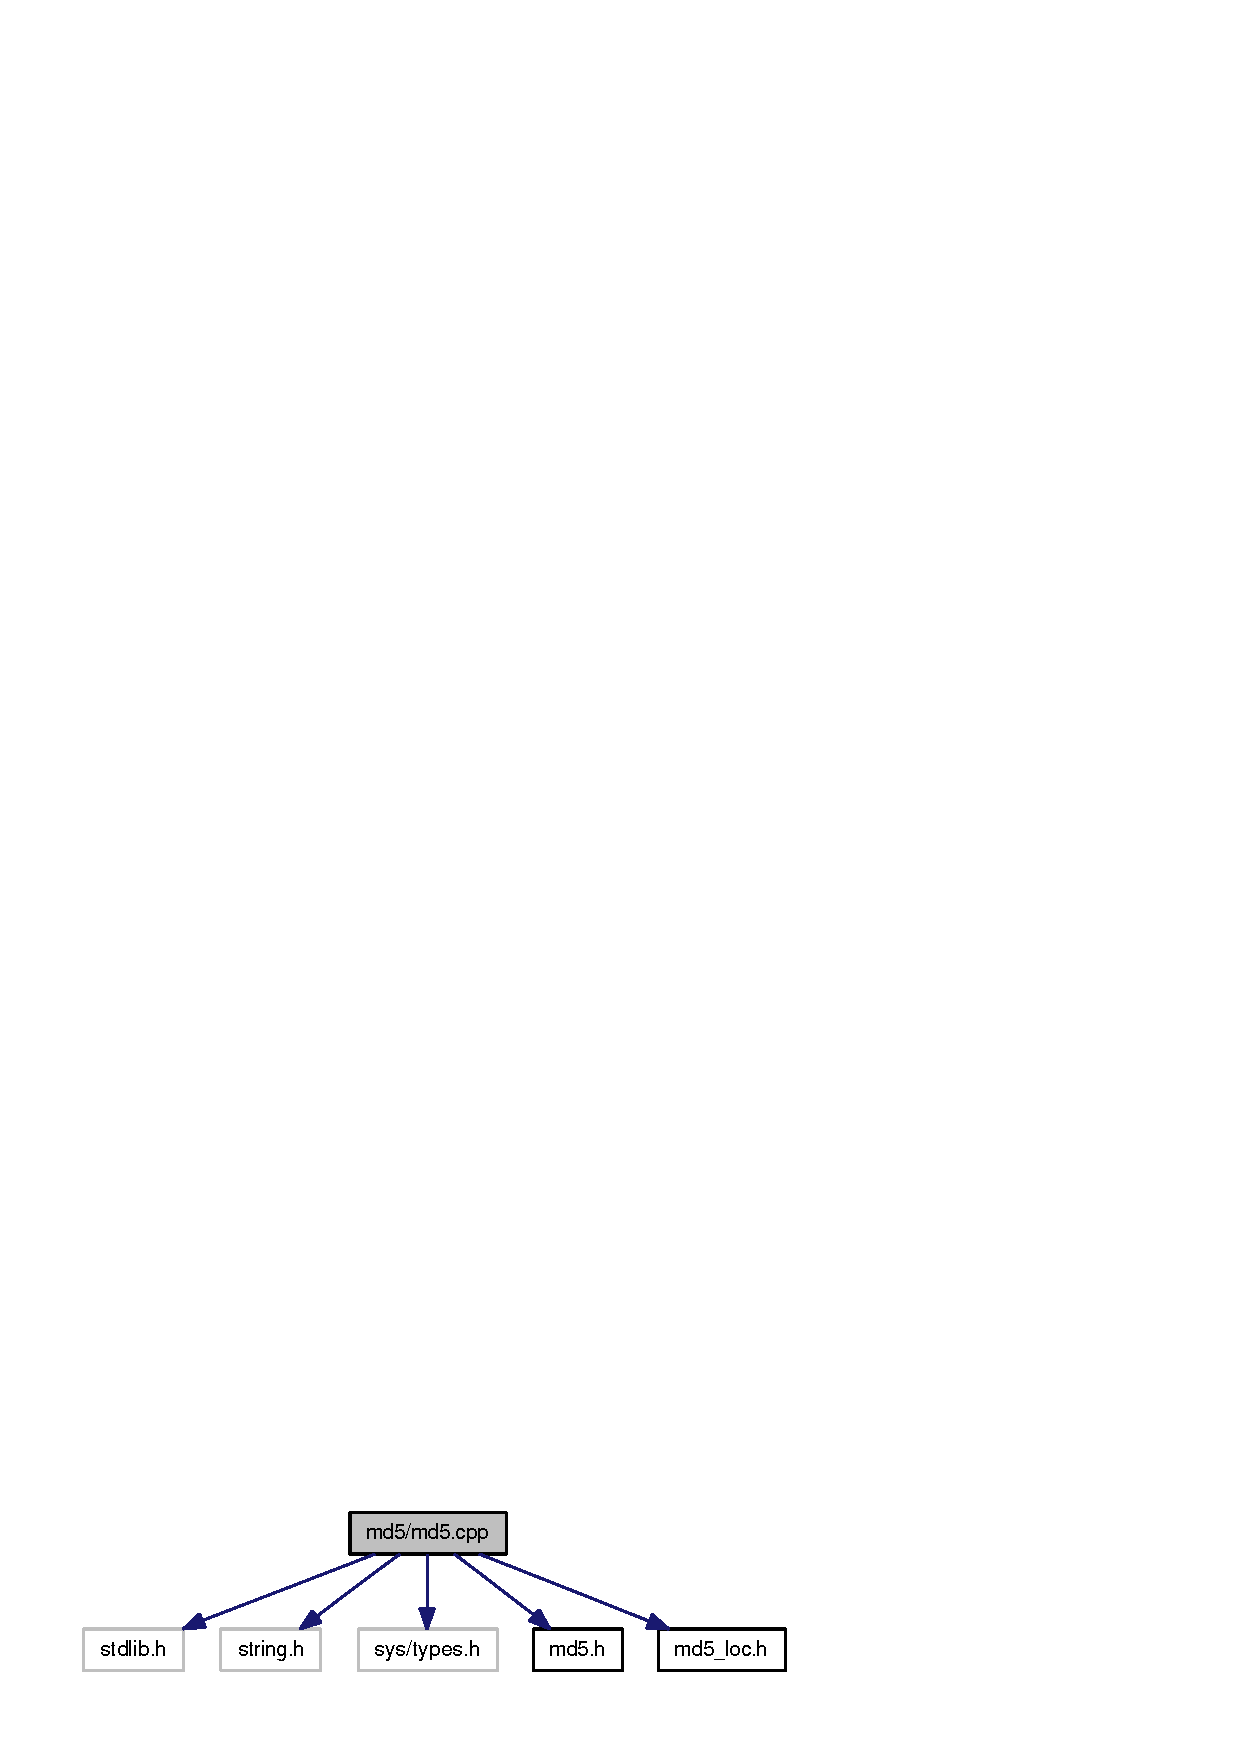
\includegraphics[width=190pt]{md5_8cpp__incl}
\end{center}
\end{figure}
\subsection*{Functions}
\begin{CompactItemize}
\item 
void \hyperlink{md5_8cpp_4534cfa15307cc94f1e557fb6238698e}{md5\_\-init} (\hyperlink{structmd5__t}{md5\_\-t} $\ast$md5\_\-p)
\item 
void \hyperlink{md5_8cpp_39eb2828c65f0846e6894a04df859f5c}{md5\_\-process} (\hyperlink{structmd5__t}{md5\_\-t} $\ast$md5\_\-p, const void $\ast$buffer, const unsigned int buf\_\-len)
\item 
void \hyperlink{md5_8cpp_11ca5c562ccb658385f45552cd840a2c}{md5\_\-finish} (\hyperlink{structmd5__t}{md5\_\-t} $\ast$md5\_\-p, void $\ast$signature)
\item 
void \hyperlink{md5_8cpp_f5de8c04dba53defbfbdd955ca7d19ab}{md5\_\-buffer} (const char $\ast$buffer, const unsigned int buf\_\-len, void $\ast$signature)
\item 
void \hyperlink{md5_8cpp_30e614459448b9ac45c84793392eea91}{md5\_\-sig\_\-to\_\-string} (void $\ast$signature, char $\ast$str, const int str\_\-len)
\item 
void \hyperlink{md5_8cpp_5f13b2aafa1b2ccc8cda48990711c5b7}{md5\_\-sig\_\-from\_\-string} (void $\ast$signature, const char $\ast$str)
\end{CompactItemize}


\subsection{Detailed Description}
Diese Funktionen liefern die Moeglichkeit, einen MD5-Hash eines beliebigen String zu generieren. 

\begin{Desc}
\item[Version:]1.7 \end{Desc}
\begin{Desc}
\item[Date:]05.03.2006 \end{Desc}
\begin{Desc}
\item[Author:]Gray Watson \end{Desc}


Definition in file \hyperlink{md5_8cpp-source}{md5.cpp}.

\subsection{Function Documentation}
\hypertarget{md5_8cpp_f5de8c04dba53defbfbdd955ca7d19ab}{
\index{md5.cpp@{md5.cpp}!md5\_\-buffer@{md5\_\-buffer}}
\index{md5\_\-buffer@{md5\_\-buffer}!md5.cpp@{md5.cpp}}
\subsubsection[md5\_\-buffer]{\setlength{\rightskip}{0pt plus 5cm}md5\_\-buffer (const char $\ast$ {\em buffer}, \/  const unsigned int {\em buf\_\-len}, \/  void $\ast$ {\em signature})}}
\label{md5_8cpp_f5de8c04dba53defbfbdd955ca7d19ab}


DESCRIPTION:

This function is used to calculate a MD5 signature for a buffer of bytes. If you only have part of a buffer that you want to process then md5\_\-init, md5\_\-process, and md5\_\-finish should be used.

\begin{Desc}
\item[Returns:]None.\end{Desc}
\begin{Desc}
\item[Parameters:]
\begin{description}
\item[{\em buffer}]A buffer of bytes whose MD5 signature we are calculating.\item[{\em buf\_\-len}]The length of the buffer.\item[{\em signature}]A 16 byte buffer that will contain the MD5 signature. \end{description}
\end{Desc}


Definition at line 483 of file md5.cpp.

References md5\_\-finish(), md5\_\-init(), and md5\_\-process().

Referenced by LogonDialog::on\_\-LogonButton\_\-released(), RechteAnpassen::on\_\-okButton\_\-released(), PasswordChangeDialog::on\_\-okButton\_\-released(), and NeuerUserDialog::on\_\-okButton\_\-released().

Here is the call graph for this function:\nopagebreak
\begin{figure}[H]
\begin{center}
\leavevmode
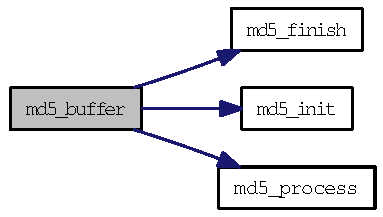
\includegraphics[width=110pt]{md5_8cpp_f5de8c04dba53defbfbdd955ca7d19ab_cgraph}
\end{center}
\end{figure}
\hypertarget{md5_8cpp_11ca5c562ccb658385f45552cd840a2c}{
\index{md5.cpp@{md5.cpp}!md5\_\-finish@{md5\_\-finish}}
\index{md5\_\-finish@{md5\_\-finish}!md5.cpp@{md5.cpp}}
\subsubsection[md5\_\-finish]{\setlength{\rightskip}{0pt plus 5cm}md5\_\-finish ({\bf md5\_\-t} $\ast$ {\em md5\_\-p}, \/  void $\ast$ {\em signature})}}
\label{md5_8cpp_11ca5c562ccb658385f45552cd840a2c}


DESCRIPTION:

Finish a progressing MD5 calculation and copy the resulting MD5 signature into the result buffer which should be 16 bytes (MD5\_\-SIZE). After this call, the MD5 structure is invalid.

\begin{Desc}
\item[Returns:]None.\end{Desc}
\begin{Desc}
\item[Parameters:]
\begin{description}
\item[{\em md5\_\-p}]Pointer to MD5 structure which we are finishing.\item[{\em signature}]A 16 byte buffer that will contain the MD5 signature. \end{description}
\end{Desc}


Definition at line 399 of file md5.cpp.

References MAX\_\-MD5\_\-UINT32, MD5\_\-BLOCK\_\-SIZE, md5\_\-t::md\_\-buf\_\-len, md5\_\-t::md\_\-buffer, and md5\_\-t::md\_\-total.

Referenced by md5\_\-buffer().\hypertarget{md5_8cpp_4534cfa15307cc94f1e557fb6238698e}{
\index{md5.cpp@{md5.cpp}!md5\_\-init@{md5\_\-init}}
\index{md5\_\-init@{md5\_\-init}!md5.cpp@{md5.cpp}}
\subsubsection[md5\_\-init]{\setlength{\rightskip}{0pt plus 5cm}md5\_\-init ({\bf md5\_\-t} $\ast$ {\em md5\_\-p})}}
\label{md5_8cpp_4534cfa15307cc94f1e557fb6238698e}


DESCRIPTION:

Initialize structure containing state of MD5 computation. (RFC 1321, 3.3: Step 3). This is for progressive MD5 calculations only. If you have the complete string available, md5\_\-buffer should be used. md5\_\-process should be called for each bunch of bytes and after the last process call, md5\_\-finish should be called to get the signature.

\begin{Desc}
\item[Returns:]None.\end{Desc}
\begin{Desc}
\item[Parameters:]
\begin{description}
\item[{\em md5\_\-p}]Pointer to md5 structure that we are initializing. \end{description}
\end{Desc}


Definition at line 294 of file md5.cpp.

References md5\_\-t::md\_\-A, md5\_\-t::md\_\-B, md5\_\-t::md\_\-buf\_\-len, md5\_\-t::md\_\-C, md5\_\-t::md\_\-D, and md5\_\-t::md\_\-total.

Referenced by md5\_\-buffer(), and LogonDialog::on\_\-LogonButton\_\-released().\hypertarget{md5_8cpp_39eb2828c65f0846e6894a04df859f5c}{
\index{md5.cpp@{md5.cpp}!md5\_\-process@{md5\_\-process}}
\index{md5\_\-process@{md5\_\-process}!md5.cpp@{md5.cpp}}
\subsubsection[md5\_\-process]{\setlength{\rightskip}{0pt plus 5cm}md5\_\-process ({\bf md5\_\-t} $\ast$ {\em md5\_\-p}, \/  const void $\ast$ {\em buffer}, \/  const unsigned int {\em buf\_\-len})}}
\label{md5_8cpp_39eb2828c65f0846e6894a04df859f5c}


DESCRIPTION:

This function is used to progressively calculate a MD5 signature some number of bytes at a time. If you have the complete string available, md5\_\-buffer should be used. The MD5 structure should have been initialized with md5\_\-init and after the last process call, md5\_\-finish should be called to get the results.

\begin{Desc}
\item[Returns:]None.\end{Desc}
\begin{Desc}
\item[Parameters:]
\begin{description}
\item[{\em md5\_\-p}]Pointer to MD5 structure which we are progressively updating.\item[{\em buffer}]A buffer of bytes whose MD5 signature we are calculating.\item[{\em buf\_\-len}]The length of the buffer. \end{description}
\end{Desc}


Definition at line 329 of file md5.cpp.

References BLOCK\_\-SIZE\_\-MASK, MD5\_\-BLOCK\_\-SIZE, md5\_\-t::md\_\-buf\_\-len, and md5\_\-t::md\_\-buffer.

Referenced by md5\_\-buffer().\hypertarget{md5_8cpp_5f13b2aafa1b2ccc8cda48990711c5b7}{
\index{md5.cpp@{md5.cpp}!md5\_\-sig\_\-from\_\-string@{md5\_\-sig\_\-from\_\-string}}
\index{md5\_\-sig\_\-from\_\-string@{md5\_\-sig\_\-from\_\-string}!md5.cpp@{md5.cpp}}
\subsubsection[md5\_\-sig\_\-from\_\-string]{\setlength{\rightskip}{0pt plus 5cm}md5\_\-sig\_\-from\_\-string (void $\ast$ {\em signature}, \/  const char $\ast$ {\em str})}}
\label{md5_8cpp_5f13b2aafa1b2ccc8cda48990711c5b7}


DESCRIPTION:

Convert a MD5 signature from a hexadecimal string representation into a 16 byte buffer.

\begin{Desc}
\item[Returns:]None.\end{Desc}
\begin{Desc}
\item[Parameters:]
\begin{description}
\item[{\em signature}]A 16 byte buffer that will contain the MD5 signature.\item[{\em str}]A string of charactes which \_\-must\_\- be at least 32 bytes long (2 characters per MD5 byte). \end{description}
\end{Desc}


Definition at line 565 of file md5.cpp.

References HEX\_\-STRING, and MD5\_\-SIZE.\hypertarget{md5_8cpp_30e614459448b9ac45c84793392eea91}{
\index{md5.cpp@{md5.cpp}!md5\_\-sig\_\-to\_\-string@{md5\_\-sig\_\-to\_\-string}}
\index{md5\_\-sig\_\-to\_\-string@{md5\_\-sig\_\-to\_\-string}!md5.cpp@{md5.cpp}}
\subsubsection[md5\_\-sig\_\-to\_\-string]{\setlength{\rightskip}{0pt plus 5cm}md5\_\-sig\_\-to\_\-string (void $\ast$ {\em signature}, \/  char $\ast$ {\em str}, \/  const int {\em str\_\-len})}}
\label{md5_8cpp_30e614459448b9ac45c84793392eea91}


DESCRIPTION:

Convert a MD5 signature in a 16 byte buffer into a hexadecimal string representation.

\begin{Desc}
\item[Returns:]None.\end{Desc}
\begin{Desc}
\item[Parameters:]
\begin{description}
\item[{\em signature}]a 16 byte buffer that contains the MD5 signature.\item[{\em str}]a string of charactes which should be at least 33 bytes long (2 characters per MD5 byte and 1 for the NULL).\item[{\em str\_\-len}]the length of the string. \end{description}
\end{Desc}


Definition at line 519 of file md5.cpp.

References HEX\_\-STRING, and MD5\_\-SIZE.